\documentclass[12pt,letterpaper]{hmcpset}
\usepackage[margin=1in]{geometry}
\usepackage{graphicx}
\usepackage{enumitem} % enumerate\
\newcommand{\vb}{\mathbf}
% example usage of amssymb: $\mathbb{Z}$
% amsmath is loaded.

% info for header block in upper right hand corner
\name{}
\class{Math 19 - \phantom{07}}
\assignment{Homework \#14}
\duedate{12/9/2019}

\begin{document}

\problemlist{Colley 6.2.4, 6.2.13, 6.3.1, 6.3.25, 7.2.1, 7.2.14, 7.3.4 \\ T/F 6, 10, 8}

\begin{problem}[Colley 6.2.4]
  Verify Green's theorem for the given vector field
  \[ \vb F = M(x,y)\vb i + N(x,y)\vb j\]
  and region D by calculating both
  \[ \oint_{\partial D} M~dx + N~dy \text{ and } \iint_D (N_x - M_y) dA\]
  where $\vb F = 2y~\vb i + x~\vb j$
  and D is the semicircular region $x^2 + y^2 \leq a^2$, $y \geq 0$.
\end{problem}
\clearpage

\begin{problem}[Colley 6.2.13]
  Evaluate $\oint_C \left( x^4y^5 - 2y \right)dx + \left( 3x + x^5y^4 \right)dy$, where $C$ is the oriented curve pictured in Figure 6.29.
  \[ 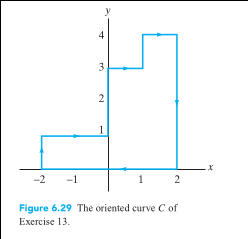
\includegraphics[width=0.4\textwidth]{assets/14_1.png} \]
\end{problem}
\clearpage

\begin{problem}[Colley 6.3.1]
  Consider the line integral $\int_C z^2~dx + 2y~dy + xz~dz$.
  \begin{enumerate}[label=(\alph*)]
  \item Evaluate this integral, where $C$ is the line segment from $(0, 0, 0)$ to $(1, 1, 1)$.
  \item Evaluate this integral, where $C$ is the path from $(0, 0, 0)$ to $(1, 1, 1)$ parameterized by $\vb x(t) = \left( t, t^2, t^3 \right), 0 \leq t \leq 1$.
  \item Is the vector field $\vb F = z^2~\vb i + 2y~\vb j + xz~\vb k$ conservative? Why or why not?
  \end{enumerate}
\end{problem}
\clearpage

\begin{problem}[Colley 6.3.25]
  Let $\vb F = x^2~\vb i + \cos y \sin z ~\vb j + \sin y \cos z ~\vb k$.
  \begin{enumerate}[label=(\alph*)]
  \item Show that $\vb F$ is conservative and find a scalar potential function $f$ for $\vb F$.
  \item Evaluate $\int_x \vb F \cdot d\vb s$ along the path $\vb x: [0,1] \to \vb R^3,~\vb x(t) = \left( t^2 + 1, e^t, e^{2t} \right)$
  \end{enumerate}
\end{problem}
\clearpage

\begin{problem}[Colley 7.2.1]
  Let $\vb X(s,t) = (s, s + t, t),\quad 0\leq s \leq 1, \quad 0 \leq t \leq 2$.
  Find
  \[ \iint_{\vb X} \left( x^2 + y^2 + z^2 \right)dS.\]
\end{problem}
\clearpage

\begin{problem}[Colley 7.2.14]
  Let $S$ denote the closed cylinder with bottom given by $z = 0$, top given by $z = 4$, and lateral surface given by the equation $x^2 + y^2 = 9$.
  Orient $S$ with outward normals.
  Determine the given vector surface integral
  \[ \iint_S \left( x~\vb i + y~\vb j\right)\cdot d\vb S \]
\end{problem}
\clearpage

\begin{problem}[Colley 7.3.4]
  Verify Stoke's theorem for the given surface and  vector field: \\
  $S$ is defined by $x^2 + y^2 + z^2 = 4$, $z \leq 0$, oriented by downward normal;
  \[ \vb F = (2y - z)\vb i + (x + y^2 - z)\vb j + (4y -3x)\vb k. \]
\end{problem}
\clearpage

\begin{problem}[Colley 7 T/F]
  \begin{enumerate}
    \addtocounter{enumi}{5}
  \item If $S$ is the unit sphere centered at the origin, then $\iint_S x^3~dS = 0$.
    \addtocounter{enumi}{3}
  \item $\iint_S (-y\vb i + x\vb j)\cdot d\vb S = 0$, where $S$ is the cylinder $x^2 + y^2 = 9$, $0 \leq z \leq 5$.
    \addtocounter{enumi}{7}
  \item $\iint_S \nabla \times \vb F \cdot d\vb S$ has the same value for all piecewise smooth, oriented surfaces S that have the same boundary curve $C$.
  \end{enumerate}
\end{problem}


\end{document}
